\documentclass[../main.tex]{subfiles}
\begin{document}

\section{Dynamic Movement Primitives  \\ \normalfont\normalsize\texttt{Bjarke Larsen}}
\label{sec:DMP}
The following section describes Dynamic Movement Primitives (DMP).
%Before dwelling into Dynamic Movement Primitives (DMP) a short motivation is presented.

\begin{figure}[H]
    \centering
         \includegraphics[width=0.50\textwidth]{figures/DMP/demonstration.png}
     \caption{Trajectory demonstration, which is handed to the DMPs.}
     \label{fig:DMP:demo}
\end{figure}
DMPs provide the option to fit a function to a discrete recording of a trajectory. In \autoref{fig:DMP:demo} a recorded trajectory is shown, which the end effector should follow from the initial position to the goal position. The idea of DMP's is to generalize learning from demonstration, in a way that allows for time scaling and dynamic modification of the trajectory.
By recording the trajectory as coordinates for the end effector in 3D space instead of recording the joint values, it allows for modification of the path based on the environment. This could be modification of the goal coordinates or dynamic avoidance of obstacles, of which avoidance of a moving obstacle will be explored in \autoref{sec:avoidance}.

%Instead of recording the joint values directly and replaying the sequence of joint values, the idea of DMPs is to generalize the demonstration, which allows for time scaling, altering the goal position and furthermore, DMPs is a framework which allows for easy expansion to include obstacle avoidance, which will be explored in \autoref{sec:avoidance}.

The idea of Dynamic Movement Primitives (DMP) is to use an analytically well-understood dynamical system that will converge towards a specific goal point \cite{ijspeert_dynamical_2013} and adding a nonlinear forcing term making the manipulator achieve a desired behavior. A spring-damper system with a forcing term is used:
\begin{align} \label{eq:system:transformation_1}
    \tau \dot{z} &= \alpha_z  (\beta_z ( g - x ) - z ) + f,\\
    \tau \dot{x} &= z,\label{eq:system:transformation_2}
\end{align}
The above system in \autoref{eq:system:transformation_1} is called the transformation system \cite{ijspeert_dynamical_2013}, where $\tau$ is a time constant, $\alpha_z$ and $\beta_z$ are constants used to adjust stiffness and damping. From \cite{ijspeert_dynamical_2013} choosing $\beta_z = \frac{\alpha_z}{4}$ the system is made critically damped, giving the desired features of a quick response without overshoot as $x$ converges to $g$.
The term $f$ is a forcing term. With $f$ being nonlinear, this enables a more useful behavior of the point attractor than a straight line. The forcing term $f$ is defined by,
\begin{equation} \label{eq:forcing}
    f(\chi) = \frac{\sum_{i=1}^{N} \psi_i(\chi) w_i}{\sum_{i=1}^{N} \psi_i(\chi)} \chi (g-x_0)
\end{equation}
Where $\chi$ is a phase variable used to make the system time independent. The term $g-x_0$ is a useful scaling when the distance between the goal and initial configuration is altered.
%The term $(g-x_0)$ is used to scale the forcing term when the distance of the movement is scaled \cite{ijspeert_dynamical_2013},
Finally by multiplying with $\chi$ it is ensured that the forcing term lets $x$ converge to $g$ since the nonlinearity will disappear as $\chi$ goes to $0$. %The functions $\psi_i(\chi)$ are basis functions and weighted by $w_i$, the individual basis functions $\psi_i(\chi)$ are defined by,
The nonlinear forcing term is built from a number of weighted basis functions. These basis functions essentially resemble gaussians with different means and variances. The forcing term is then built from a weighted sum of the basis functions, to imitate the recorded path. The individual basis functions $\psi_i(\chi)$ are defined by,
\begin{equation}
    \psi_i(\chi) = \text{exp}\left(-\frac{1}{2\sigma_i^2}(\chi-c_i)^2\right)
\end{equation}
Where $\sigma_i$ determines the width of the basis function and $c_i$ defines the center of the basis function. Choosing the centers for the basis functions is a matter of design. One option being to place the centers evenly along as the phase goes to zero, while another option could be to cluster the basis functions closer together based on the complexity of the trajectory for a better result with fewer basis functions.
%The basis function can either be spread evenly along the phase variable or using various techniques including placing the centers as a with density as an exponential function of the phase variable,
The phase variable, $\chi$, is used to avoid dependency on time and thus enabling time scaling. The phase variable is defined by the following first-order linear dynamic system, which is called the canonical system,
\begin{equation} \label{eq:system:canonical}
    \tau \dot{\chi} = -\alpha_\chi \chi
\end{equation}
Since this canonical system decays to zero exponentially the centers of the basis functions are placed as follows:
\begin{equation}
    c_i = \text{exp}\left(-\alpha_c \cdot \frac{i}{N}\right)
\end{equation}
Where $N$ is the total amount of basis functions and $\alpha_c$ is a positive constant. In \autoref{fig:dmp:basis} an illustration of the basis functions is shown with linear spacing and with the exponential centers resulting in an even spacing given the choice of canonical system.
\begin{figure}[H]
    \centering
    \begin{subfigure}[b]{0.48\textwidth}
        \centering
        \includegraphics[width=\textwidth]{figures/DMP/dmp_f.png}
        \caption{Centers placed linearly as a function of indice.}
        \label{fig:dmp:basis:lin}
    \end{subfigure}
    \hfill
    \begin{subfigure}[b]{0.48\textwidth}
        \centering
        \includegraphics[width=\textwidth]{figures/DMP/dmp_basis_exp.png}
        \caption{Centers of basis function placed as an exponential function of indices.}
        \label{fig:dmp:basis:exp}
    \end{subfigure}
    \caption{Visualization of the two considered ways of distributing basis function centers.}
    \label{fig:dmp:basis}
\end{figure}
To make the DMP follow the demonstration shown in \autoref{fig:DMP:demo} the weights $w_i$ in the nonlinear forcing term in \autoref{eq:forcing} needs to be adjusted. Learning these weights can be accomplished from a single demonstration using linear regression.
%To fit the DMP to the demonstration shown in \autoref{fig:DMP:demo}, the weights $w_i$ in \autoref{eq:forcing} are being adjusted to make the DMP fit to the demonstration. The learning of the weight can be done by linear regression.
From the transformation system in \autoref{eq:system:transformation_1}, the following can be seen \cite{ijspeert_dynamical_2013}:
\begin{equation}\label{eq:system:forcing}
    \tau \dot{z} -\alpha_z (\beta_z (g-x) - z) = f
\end{equation}
By inserting the known information from the demonstration in the left side,
\begin{equation} \label{eq:transformation:demo}
    \tau^2 \ddot{x}_{demo} - \alpha_z(\beta_z(g-x_{demo}) - \tau \dot{x}_{demo}) = f_{target}
\end{equation}
The objective is now to determine the weights, $w_i$, that makes the trajectory $f$ come as close to $f_{target}$ as possible.
%The objective is now to find weights, $w_i$, such that $f$ comes as close as possible to $f_{target}$.
This is now written as a system of linear equations. First the matrix $\boldsymbol{\Psi}$ is defined, which simply contains the $N$ basis functions along the rows and has $K$ rows, where $K$ is the number of samples in the demonstration. Along with the matrix of basis functions a vector of all the weights is also defined,
\begin{equation}
    \underset{(K \times N)}{\boldsymbol{\Psi}} = \begin{bmatrix} \psi_0 & \psi_1 & \dots & \psi_N \\ \psi_0 & \psi_1 & \dots & \psi_N \\ \vdots & \vdots & \vdots & \vdots \\\psi_0 & \psi_1 & \dots & \psi_N \end{bmatrix}, \quad \underset{(N\times 1)}{\boldsymbol{W}} = \begin{bmatrix} w_0 \\ w_1 \\ \vdots \\ w_N \end{bmatrix} 
\end{equation}
Finally, \autoref{eq:transformation:demo} is put on matrix form,
\begin{equation}
    \underset{(K \times 1)}{\boldsymbol{F}} = \begin{bmatrix} f_{target,0} \\ f_{target,1} \\ \vdots \\ f_{target,K} \end{bmatrix}
\end{equation}
The system of linear equations to be solved using least squares is then,
\begin{equation}\label{eq:system:sole}
    \boldsymbol{\Psi}\boldsymbol{W} = \boldsymbol{F}
\end{equation}

Based on a trial and error approach the following was determined to be used: $\alpha_z = 48$, center of basis function placed with increasing density as $\chi$ approaches $0$ to accommodate the choice of canonical system. The basis function parameter $\sigma$ was chosen based on the handed template \cite{inigo},
\begin{equation}
    \sigma_i = c_{i+1} - c_i
\end{equation}
Which indicates that the width of the basis functions decreases as the density increases.

By fitting the DMPs to the demonstration in \autoref{fig:DMP:demo}, the following is achieved
\begin{figure}[H]
    \centering
    \begin{subfigure}[b]{0.48\textwidth}
        \centering
        \includegraphics[width=\textwidth]{figures/DMP/dmp.png}
        \caption{Dynamic Movement Primitive fitted to the demonstration shown in cartesian space.}
        \label{fig:dmp:fit:cartesian}
    \end{subfigure}
    \hfill
    \begin{subfigure}[b]{0.48\textwidth}
        \centering
        \includegraphics[width=\textwidth]{figures/DMP/dmp_fit.png}
        \caption{DMP fitted to the demonstration shown in X, Y and Z axes.}
        \label{fig:dmp:fit:xyz}
    \end{subfigure}
    \caption{Results for fitting the DMP to the demonstration with $\tau = \frac{1}{500} N_{demo}$, where $N_{demo}$ is amount of samples in demonstration, and with 30 basis functions.}
    \label{fig:dmp:fit}
\end{figure}

\subsection{Including Rotation in the DMP \\ \normalfont\normalsize\texttt{Bjarke Larsen}} \label{subsec:dmp_with_rotation}
In addition to controlling the end effector position as presented in \autoref{sec:DMP} it is possible to also control the orientation of the end effector in a similar way. Here we will focus on the use of quaternions for describing the orientation of the end effector since this gives a robust representation with few variables. As presented in \cite{ude_orientation_2014}, analogous to \autoref{eq:system:transformation_1} and \ref{eq:system:transformation_2} a system can be set up. In the following $\mathbf{\bar{q}}$ denotes the quaternion conjugate and * denotes the quaternion product.
\begin{align}\label{eq:system:quaternion:transformation}
    \tau\dot{\boldsymbol{\eta}} &= \alpha_z(\beta_z\cdot2\cdot log(\mathbf{g}_0*\mathbf{\bar{q}})-\boldsymbol{\eta})+\mathbf{f}(x)\\
    \tau\dot{\mathbf{q}} &= \frac{1}{2}\boldsymbol{\eta}*\mathbf{q}\label{eq:system:quaternion:transformation_2}
\end{align}
Where \autoref{eq:system:quaternion:transformation_2} has to be integrated in the following way \cite{ude_orientation_2014}.
\begin{equation}
    \mathbf{q}(t+\delta t)=exp\left(\frac{\delta t}{2}\frac{\boldsymbol{\eta}(t)}{\tau}\right) * \mathbf{q}(t)
\end{equation}
The main reason the system in Equations \ref{eq:system:quaternion:transformation} and \ref{eq:system:quaternion:transformation_2} differs from what seen previously is that while the variables for position are independent they are not independent for rotations.
This means that learning the weights for the basis functions as seen in Equation \ref{eq:transformation:demo} is written on the following form.
\begin{equation}
    \tau^2\dot{\boldsymbol{\omega}}_{demo}-\alpha_z(\beta_z\cdot2\cdot log(\mathbf{g}_0*\bar{\mathbf{q}}_{demo})-\tau\cdot{\boldsymbol{\omega}}_{demo}) = \mathbf{f}_{target}
\end{equation}
Here $2log(\mathbf{g}_0*\mathbf{\bar{q}}_{demo})$ is the angular velocity in unit time between the current demonstrated $\mathbf{q}_i$ and the goal orientation. $\boldsymbol{\omega}_{demo}$ is the angular velocity at the current time calculated as $2log(\mathbf{q}_{i+1}*\mathbf{q}_i)$ and $\boldsymbol{\dot{\omega}}_{demo}$ is the angular acceleration at the current time. Since the angular velocity is given as a quaternion with zero scalar part it is only necessary to learn three weights so the minimization problem is entirely analogous to the problem solved for position in Equation \ref{eq:system:sole}. Since the problem of finding the correct weights is the same, $\mathbf{f}$ is the same as in Equation \ref{eq:system:forcing} with the only exception being the scaling term $(g_0-x)$ being a 3x3 matrix with the quaternion velocity.\\
The result from implementing the DMP for orientation based on modifying the handed template \cite{inigo} to accommodate quaternions, with 100 basis functions, is seen in \autoref{fig:dmp:quaternion}.
\begin{figure}[H]
    \centering
    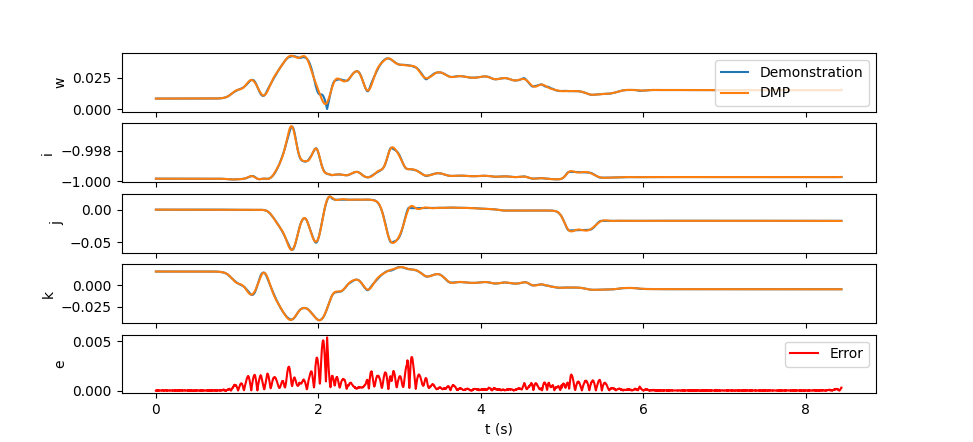
\includegraphics[width=\textwidth]{figures/DMP_quat/quat_dmp.png}
    \caption{The result from fitting the DMP to the recorded orientation.}
    \label{fig:dmp:quaternion}
\end{figure}
The four top plots in \autoref{fig:dmp:quaternion} are the individual parts of the quaternion, $w + [xi\ yj\ zk]$ The error \textit{e}, plotted at the bottom in \autoref{fig:dmp:quaternion} is calculated as the distance on the unit sphere between the recorded data and the fitted data.

\end{document}